\documentclass{article}
\usepackage[utf8]{inputenc}
\usepackage[margin = 1 in]{geometry}
\usepackage{listings}
\usepackage{xcolor}
\usepackage{booktabs}
\usepackage{graphicx}


\definecolor{codegreen}{rgb}{0, 0.6, 0}
\definecolor{codegray}{rgb}{0.5, 0.5, 0.5}
\definecolor{codepurple}{rgb}{0.58, 0, 0.82}
\definecolor{backcolour}{rgb}{0.95, 0.95, 0.92}

\lstdefinestyle{mystyle}
{
	backgroundcolor =\color{backcolour},
	commentstyle =\color{codegreen},
	keywordstyle =\color{magenta},
	numberstyle =\tiny\color{codegray},
	stringstyle =\color{codepurple},
	basicstyle =\ttfamily\footnotesize,
	breakatwhitespace = false,
	breaklines = true,
	captionpos = b,
	keepspaces = true,
	numbers = left,
	numbersep = 5pt,
	showspaces = false,
	showstringspaces = false,
	showtabs = false,
	tabsize = 2
}

\lstset{style = mystyle}
\begin{document}
\begin{titlepage} % Suppresses displaying the page number on the title page and the subsequent page counts as page 1

\raggedleft\rule{1pt}{\textheight} % Vertical line
\hspace{0.05\textwidth} % Whitespace between the vertical line and title page text
\parbox[b]{0.75\textwidth}
	{% Paragraph box for holding the title page text, adjust the width to move the title page left or right on the page

            {\Huge\bfseries MIT World Peace University \\[0.5\baselineskip] \ SET}\\[2\baselineskip] % Title
            {\large\textit{Assignment 7}}\\[4\baselineskip] % Subtitle or further description
            {\Large\textsc{Naman Soni Roll No. 10}} % Author name, lower case for consistent small caps

   \vspace{0.5\textheight} % Whitespace between the title block and the publisher
   }

\end{titlepage}
\tableofcontents
\pagebreak
\section{\textbf{Aim}}
Object Oriented Analysis and design using UML diagrams: Component diagram, deployment diagram using Open Source Tool.
The tasks we have to do are:
\begin{enumerate}
    \item You will have to identify the main entities (objects) for this system.
    \item You will have to find out the messages between these objects for communication diagram.
    \item You will have to find the necessary attributes and functions that need to be associated with each object to implement the functionality mentioned above.
    \item You will make a final comprehensive diagram showing all objects and their messages.
\end{enumerate}

\section{\textbf{Objectives}}
\begin{itemize}
    \item To learn the relationships and notions of Component diagram.
    \item To learn the relationships and notions of Deployment diagram.
\end{itemize}
\section{\textbf{Problem Statement}}
\textbf{Draw Component Diagram for the following problem statement:}The restaurant industry is a fast-paced environment that requires efficient management of resources to ensure timely and quality service. In the traditional restaurant setting, the ordering process, food preparation, and inventory management are carried out manually, leading to errors, delays, and inefficiencies.
\section{\textbf{Theory}}
\subsection{\textbf{Component Diagram}}
A component diagram is a type of structural diagram in UML (Unified Modeling Language) that represents the structure and organization of the components that make up a system. It provides a high-level view of the system's architecture, showing how the different components interact and collaborate to fulfill the system's functionality. Component diagrams are commonly used in software engineering to model complex systems and to communicate the system's structure and dependencies to stakeholders.

Here are some key points to understand about component diagrams:
\begin{enumerate}
    \item Components: Components represent the modular parts or building blocks of a system. They encapsulate the implementation details and provide specific functionalities or services. Examples of components can include software modules, libraries, frameworks, hardware devices, or subsystems. Components can be represented by rectangles with the component's name written inside.
    \item Interfaces: Interfaces define the contracts or specifications of how components can interact with each other. They define the methods, operations, or services that a component provides or requires. Interfaces can be represented by labeled lines connecting components. The provided interfaces (interfaces that the component exposes) are depicted as solid lines with an arrowhead, while required interfaces (interfaces that the component depends on) are depicted as dashed lines with an arrowhead.
    \item Relationships: Component diagrams depict the relationships and dependencies between components. Some common relationships include:
        \begin{itemize}
            \item  Dependency: It represents a relationship where one component depends on another component. It is typically shown as a dashed line with an arrowhead pointing from the dependent component to the component it depends on.
            \item  Association: It represents a relationship between components where one component is associated with or has a reference to another component. It is depicted as a solid line connecting the associated components.
            \item  Aggregation and Composition: These relationships depict the part-whole or container-contained relationships between components. Aggregation represents a relationship where one component is composed of multiple other components, while composition represents a stronger form of aggregation where the lifetime of the contained component is controlled by the container.
        \end{itemize}
    \item Deployment: Component diagrams can also show the physical deployment of components on hardware nodes or devices. This is known as a deployment diagram. It helps visualize how the components are distributed across the hardware infrastructure of the system.
    \item Communication and Collaboration: Component diagrams facilitate communication and collaboration among stakeholders by providing a clear and concise representation of the system's architecture and its components. They enable a shared understanding of the system's structure and dependencies, aiding in the design, development, and maintenance of the system.
\end{enumerate}
Component diagrams are particularly useful in complex systems where the decomposition into modular components helps manage system complexity, improve maintainability, and facilitate system integration. They serve as a blueprint for system architects, developers, and system analysts, guiding the implementation and ensuring the system's structural integrity.
\section{\textbf{Component Diagram}}
\begin{center}
    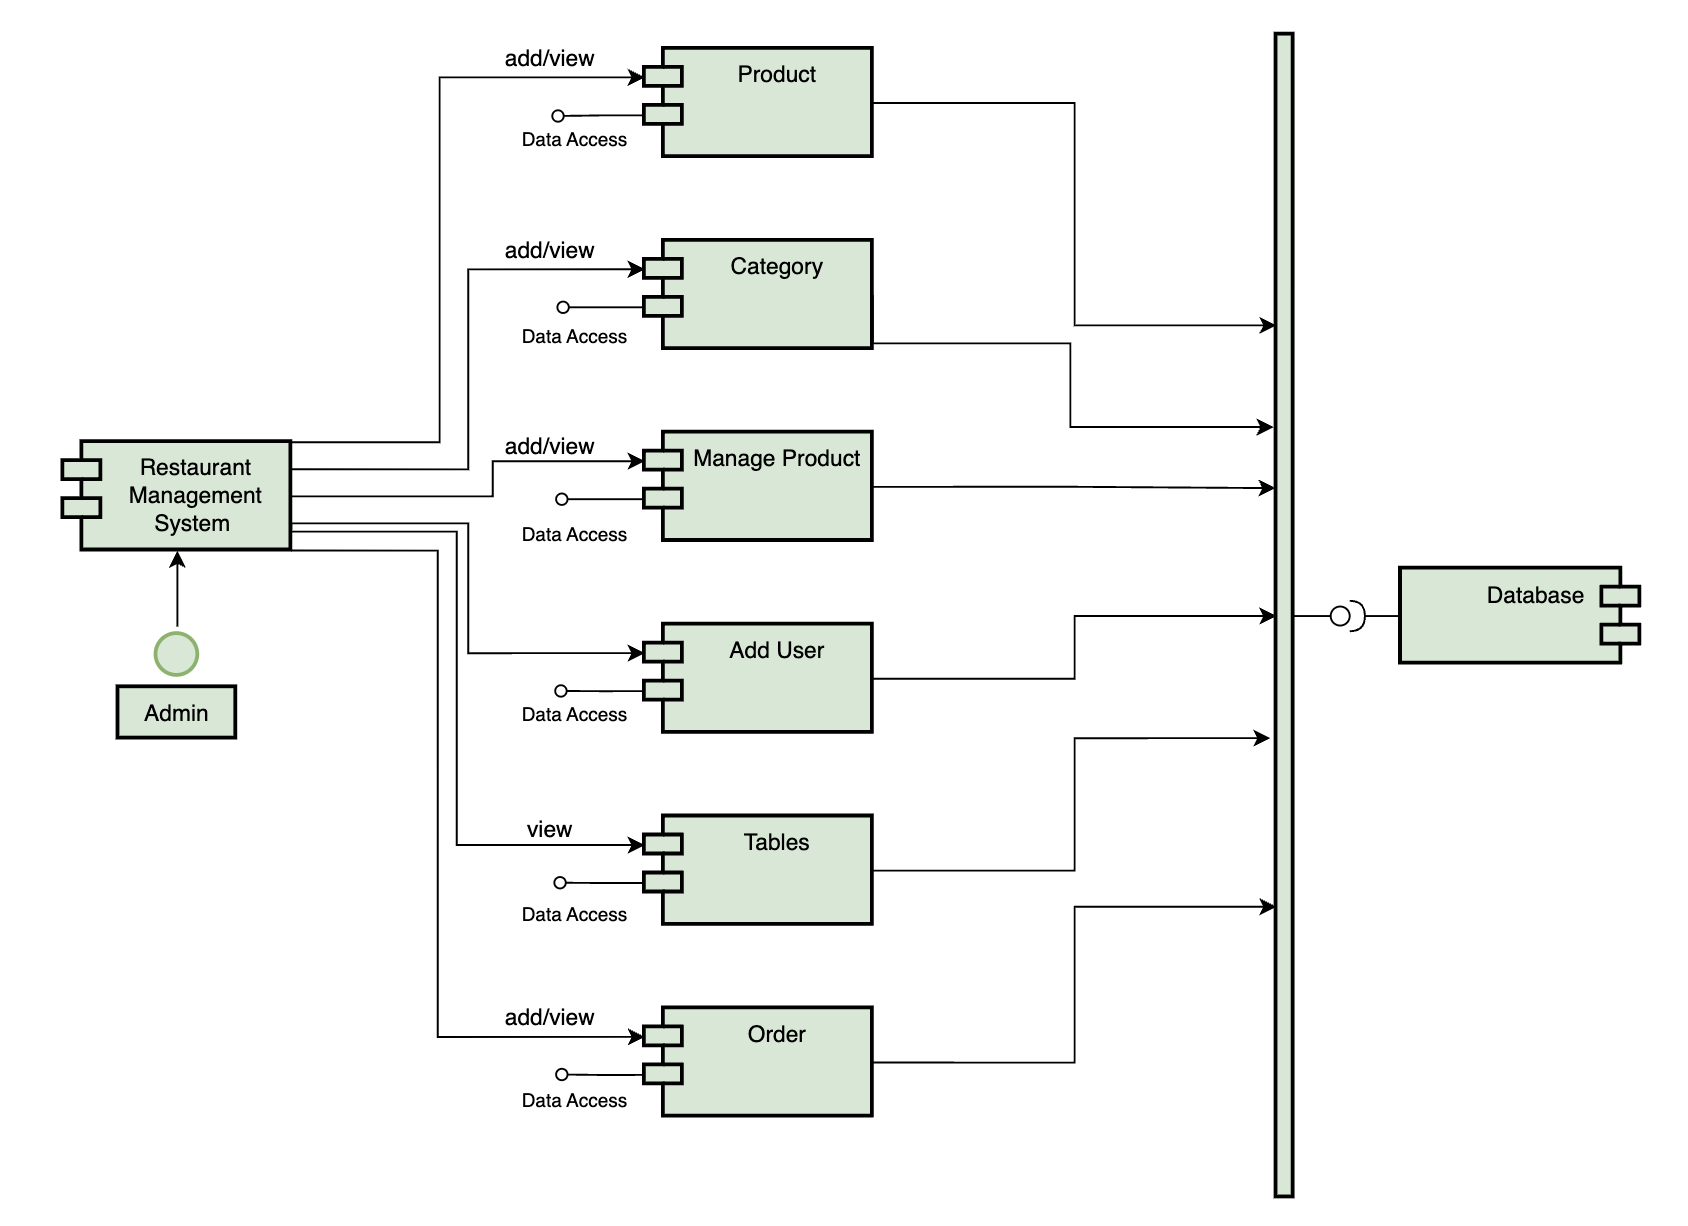
\includegraphics[scale = 0.5]{Component Diagram.png}
\end{center}
\section{\textbf{Conclusion}}
We studied about Component Diagram and how to draw it using Open Source Tool.
\section{\textbf{FAQ's}}
\subsection{\textit{The term component is sometimes a difficult one to define. First provide a
generic definition, and then provide more explicit definitions for object-
oriented and traditional software. Finally, pick three programming
languages with which you are familiar and illustrate how each defines a
component.}}
\textbf{Ans.} Generic Definition of a Component: A component is a modular and self-contained unit that encapsulates specific functionalities or behaviors. It can be considered as a building block or a reusable piece of software or hardware that can be integrated into larger systems. Components exhibit well-defined interfaces, allowing them to be easily interconnected and composed to create complex systems.\\

Explicit Definitions for Object-Oriented and Traditional Software:
\begin{enumerate}
    \item Object-Oriented Definition: In object-oriented software development, a component is a self-contained and reusable software module that encapsulates data and behaviors within a single unit. It typically corresponds to a class or a collection of closely related classes that work together to provide a specific functionality. Components in object-oriented programming emphasize encapsulation, modularity, and reusability, following principles such as information hiding and separation of concerns.
    \item Traditional Software Definition: In traditional software development, a component refers to a standalone and independent piece of software that provides specific functions or services. It can be a library, a module, or a subsystem that performs a well-defined task and can be integrated into larger software systems. Traditional software components often emphasize functionality, interoperability, and reuse across different programming languages and platforms.
\end{enumerate}
Illustration of Component Definitions in Programming Languages, here are three programming languages and how they define components:
\begin{enumerate}
    \item Java: In Java, a component can be defined as a class or a collection of related classes that provide a specific functionality. Components in Java are typically implemented using classes and interfaces. A Java component encapsulates data and methods within a class and can be instantiated, reused, and composed with other components through well-defined interfaces.
    \item Python: In Python, a component can be represented as a module or a package. A module is a file containing Python code that defines classes, functions, or variables. It serves as a self-contained unit that can be imported and used in other Python programs. Packages, on the other hand, are directories that contain multiple modules, allowing for hierarchical organization and management of components.
    \item JavaScript: In JavaScript, a component can be implemented using various approaches. One common approach is using JavaScript libraries or frameworks, such as React or Angular. These frameworks enable the development of reusable UI components that encapsulate the structure and behavior of a user interface element. JavaScript components can be composed, reused, and interact with other components to build complex web applications.
\end{enumerate}
\subsection{\textit{What is a WebApp component?}}
\textbf{Ans.} A web application component refers to a specific part or module within a web application that provides a distinct functionality or feature. It is a self-contained unit that contributes to the overall functionality, behavior, or presentation of the web application. Web application components are designed to be reusable, modular, and independent, allowing developers to build complex applications by combining and integrating these components.\\

Web application components can take different forms depending on the architecture and technologies used in the web application development. Here are a few common types of web application components:
\begin{enumerate}
    \item User Interface (UI) Components: UI components are responsible for presenting the user interface and handling user interactions. They include elements such as buttons, forms, menus, tables, and various UI controls. UI components provide visual representation and interactivity, allowing users to interact with the web application.
    \item Backend Components: Backend components handle the server-side logic and functionality of the web application. They include components responsible for data processing, business logic implementation, and integration with external services or databases. Backend components ensure the proper functioning and behavior of the web application's core functionality.
    \item Data Components: Data components manage the storage, retrieval, and manipulation of data within the web application. They can include database access components, data models, data access layers, and caching components. Data components facilitate efficient and secure data management in the web application.
    \item Communication Components: Communication components enable communication and interaction between the web application and external systems or services. They can include components responsible for API integration, message queues, real-time communication, or communication with external services such as payment gateways or social media platforms.
    \item Security Components: Security components handle various aspects of web application security, such as authentication, authorization, input validation, encryption, and protection against common security threats. They ensure that the web application is secure and protected from unauthorized access or malicious activities.
\end{enumerate}
Web application components are often designed with a modular and reusable approach, allowing developers to easily integrate, replace, or extend functionality as needed. They contribute to the separation of concerns, making the application easier to maintain, test, and scale. Component-based web application development promotes code reusability, flexibility, and efficient collaboration among developers working on different parts of the application.
\subsection{\textit{State the importance of deployment diagram.}}
\textbf{Ans.} Deployment diagrams are important in system design and development as they provide a visual representation of how software and hardware components are deployed and interconnected within a system's infrastructure. Here are some key reasons why deployment diagrams are important:
\begin{enumerate}
    \item System Architecture Visualization: Deployment diagrams offer a clear and concise representation of the physical deployment and arrangement of components in a system. They provide an overview of how the system's software and hardware components are distributed across different nodes, servers, or devices. This visualization helps stakeholders, including system architects, developers, and administrators, understand the overall system architecture and how the various components interact.
    \item Hardware and Software Mapping: Deployment diagrams depict the mapping of software components to the hardware nodes or devices on which they are deployed. This mapping shows the specific hardware resources (such as servers, computers, or devices) required to support the software components. It helps in resource planning, hardware provisioning, and ensuring that the necessary infrastructure is available to run the system effectively.
    \item System Scalability and Performance Planning: Deployment diagrams aid in system scalability and performance planning by illustrating the distribution of components across multiple nodes or servers. It helps identify potential bottlenecks, performance constraints, or single points of failure in the system architecture. By analyzing the deployment diagram, system designers can make informed decisions about load balancing, redundancy, and resource allocation to ensure optimal performance and scalability.
    \item Communication among Development Teams: Deployment diagrams serve as a communication tool among development teams, system administrators, and other stakeholders involved in the system's implementation and maintenance. They provide a common visual language to discuss and understand the system's deployment strategy, infrastructure requirements, and interconnections between components. Deployment diagrams facilitate collaboration and coordination, ensuring a shared understanding of the system's deployment across the development and operations teams.
    \item System Maintenance and Troubleshooting: Deployment diagrams aid in system maintenance and troubleshooting activities. They provide a reference for system administrators to understand the physical deployment of components and their dependencies. In case of issues or failures, deployment diagrams help pinpoint the affected components, their location, and the potential impact on the overall system. This information expedites problem identification, diagnosis, and resolution.
    \item Compliance and Security Considerations: Deployment diagrams help address compliance and security considerations by visualizing the flow of data and dependencies between components. They assist in identifying potential security risks, data access points, and compliance requirements. Deployment diagrams support the implementation of security measures, access controls, and data protection mechanisms based on the system's physical deployment.
\end{enumerate}
Overall, deployment diagrams play a crucial role in understanding, planning, and communicating the physical deployment of software and hardware components within a system. They support system design, performance optimization, collaboration, troubleshooting, and compliance, ultimately contributing to the successful implementation and operation of complex systems.
\end{document}